\section{Explicit Register Renaming}

Explicit Register Renaming uses a physical register file larger than what the ISA specifies. 
The core idea is to allocate a new physical destination register for each instruction that writes a result, resembling the Static Single Assignment (SSA) form used by compilers but implemented in hardware. 
This approach effectively eliminates the risk of WAR or WAW hazards.
\begin{figure}[H]
    \centering
    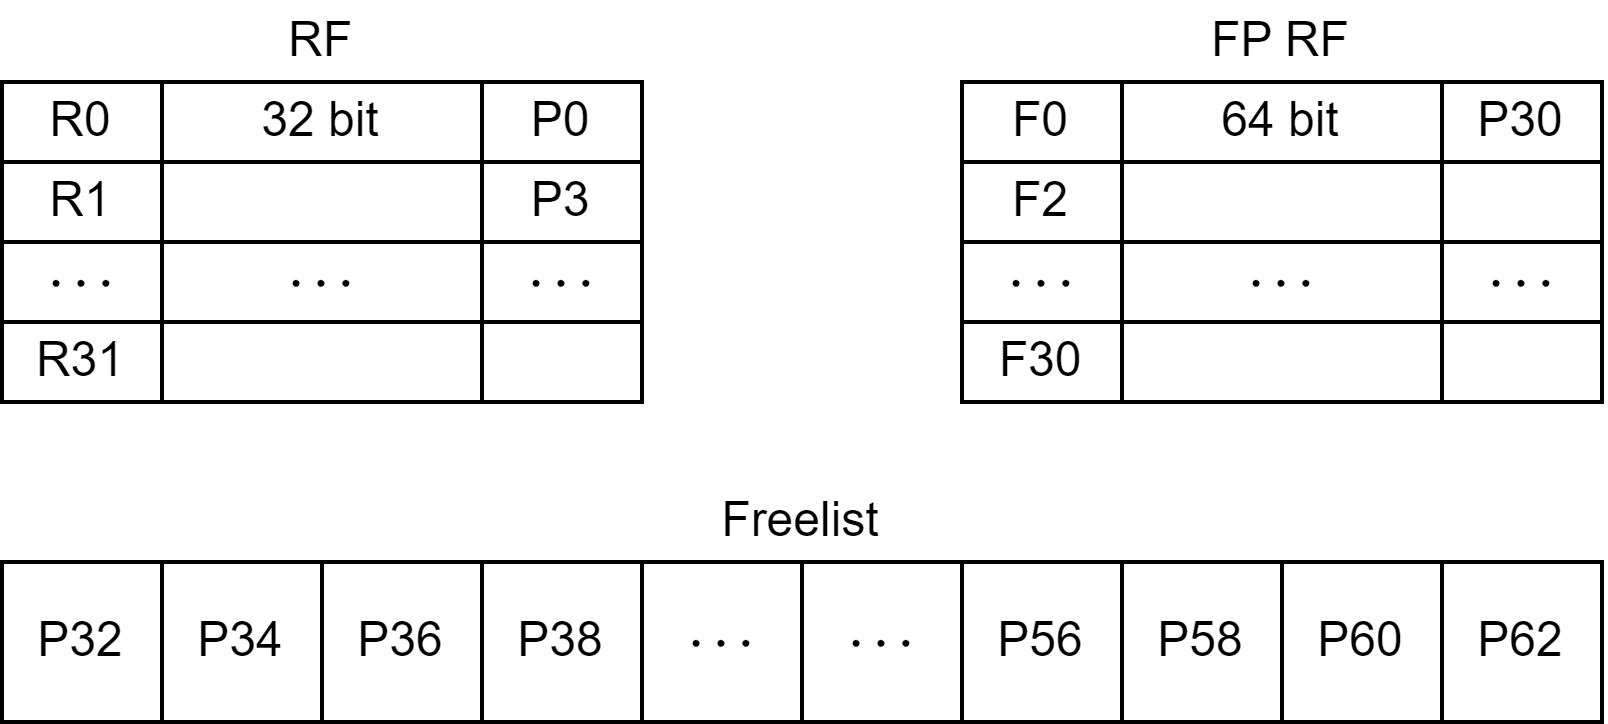
\includegraphics[width=0.5\linewidth]{images/err.png}
    \caption{Explicit Register Renaming}
\end{figure}
Expanding the physical register file beyond the ISA register file size involves the following steps:
\begin{enumerate}
    \item Upon issuance, each instruction that produces a result is assigned a new physical register from the available free list.
    \item When a physical register is no longer needed, it is returned to the free list for future use.
\end{enumerate}
Explicit Register Renaming requires maintaining a translation table that maps ISA registers to physical registers. 
When an instruction writes to a register, the corresponding entry in the translation table is updated with a new physical register from the pool. 
Physical registers are released when they are no longer used by any active instructions.
\begin{figure}[H]
    \centering
    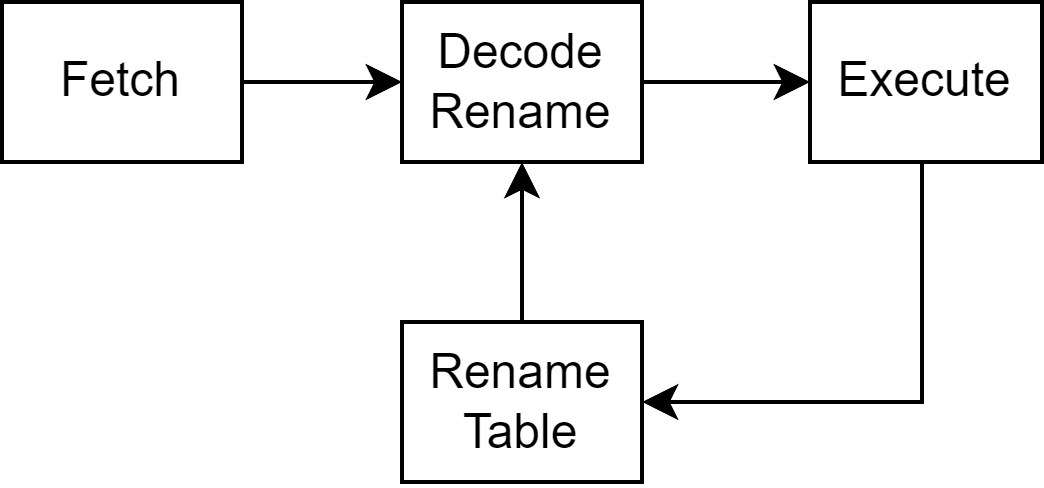
\includegraphics[width=0.4\linewidth]{images/errm.png}
    \caption{Explicit Register Renaming mechanism}
\end{figure}

In the unified physical register file approach, architectural registers are integrated into a single physical register file during the decoding stage, without accessing register values. 
FUs interact with this unified register file, accessing and updating both committed and temporary registers during execution. 
Committing an instruction involves updating the mapping of architectural registers to physical registers without moving any data.
\begin{figure}[H]
    \centering
    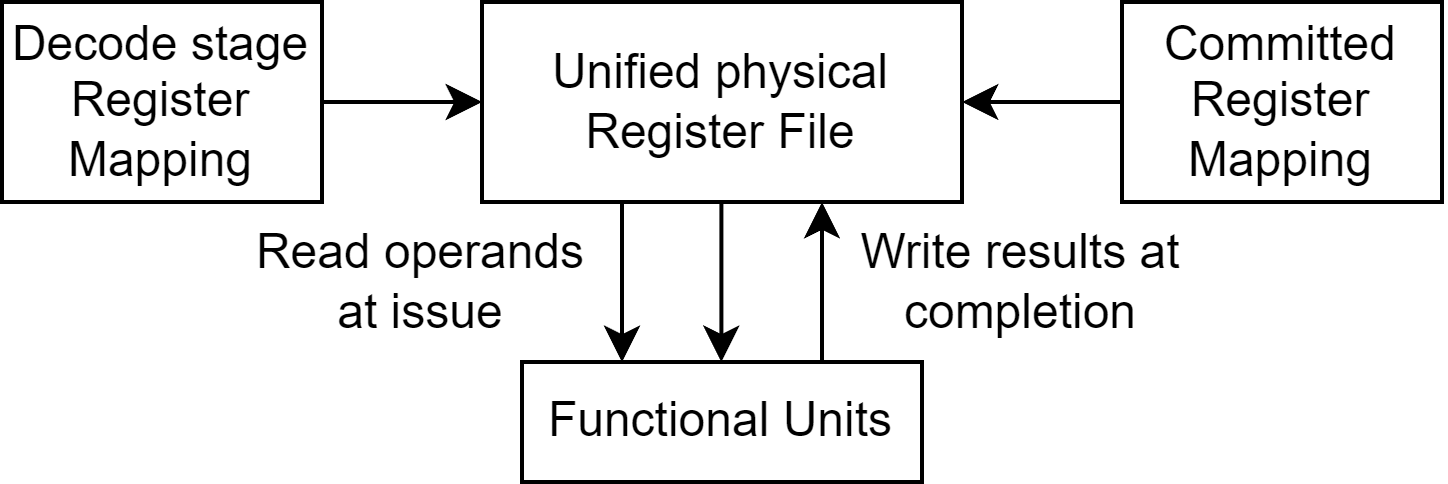
\includegraphics[width=0.5\linewidth]{images/uprf.png}
    \caption{Unified physical Register File}
\end{figure}

\subsection{Explicit Register Renaming features}
Instruction commit includes the following steps:
\begin{enumerate}
    \item Mark the mapping between an architectural register number and a physical register number as non-speculative, finalizing it.
    \item Release any physical registers used to store the previous value of the architectural register.
    \item De-allocating registers involves:
        \begin{itemize}
            \item Ensuring a physical register no longer corresponds to an architectural register and has no further outstanding uses before freeing it.
            \item A physical register remains associated with an architectural register until that register is overwritten.
            \item Checking if any source operand in the FU queue corresponds to the register. If not, the register can be de-allocated.
        \end{itemize}
        Alternatively, the processor can wait until another instruction that writes to the same architectural register commits. 
        This method might slightly prolong the usage of a physical register but is easier to implement.
\end{enumerate}

\subsection{Explicit Register Renaming structure}
Explicit Register Renaming requires specific components to manage the mapping between architectural registers and physical registers efficiently:
\begin{itemize}
    \item \textit{Renaming map}: this is a straightforward data structure that provides the mapping from architectural register numbers to corresponding physical register numbers.
        Whenever an instruction writes to an architectural register, the renaming map is updated to reflect the physical register holding the result.
    \item \textit{Instruction commit}: during the commit phase of an instruction, the renaming map is updated permanently. 
        This update indicates that the physical register holding the destination value now corresponds to the actual architectural register.
\end{itemize}
To enforce in-order commit, a ReOrder Buffer (ROB) is employed. 
The ROB ensures that instructions are committed in the same order they were fetched, despite possible out-of-order execution.
\begin{figure}[H]
    \centering
    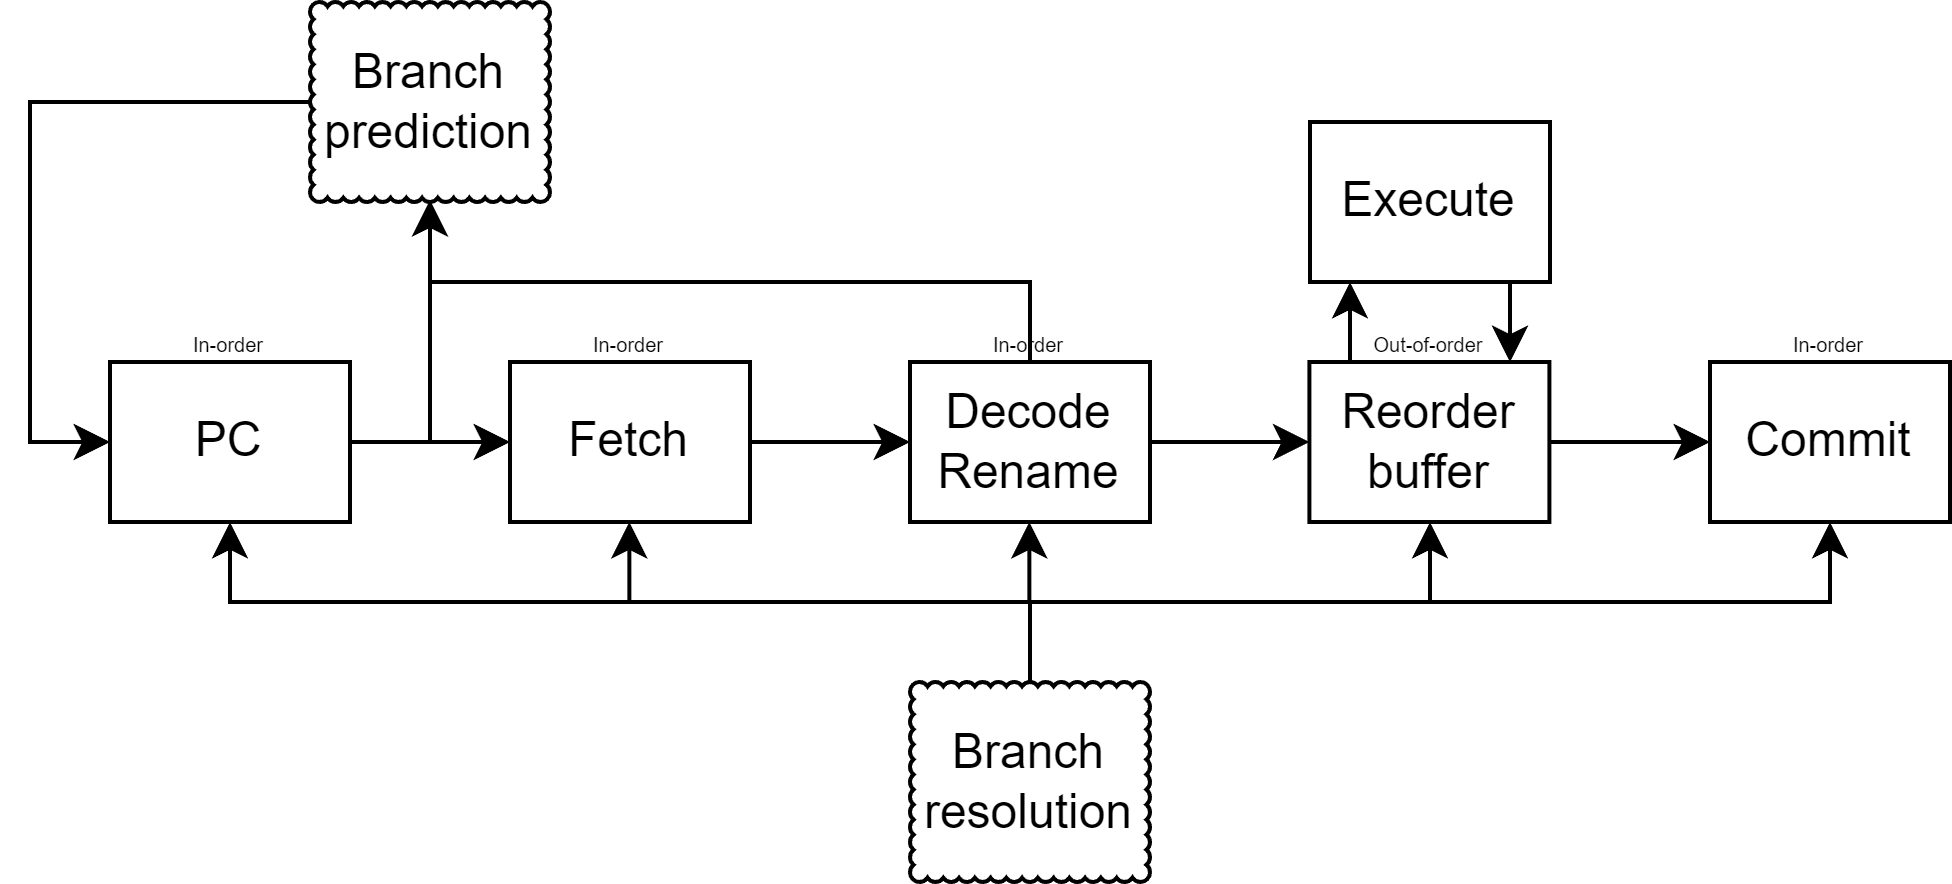
\includegraphics[width=0.5\linewidth]{images/herr.png}
    \caption{Explicit Register Renaming}
\end{figure}

Explicit Register Renaming offers several advantages:
\begin{itemize}
    \item \textit{Decoupling Renaming from scheduling}: this approach provides flexibility in pipeline design. 
        The processor can adopt various scheduling methodologies, such as issuing multiple operations per cycle or implementing algorithms like Tomasulo or Scoreboard. 
        It also allows for standard forwarding or bypassing techniques to be employed.
    \item \textit{Single Register File access}: retrieval of data from a single Register File is facilitated, eliminating the need to bypass values from the ROB. 
        This simplifies pipeline management and enhances overall efficiency.
    \item \textit{Widespread adoption}: many processors have adopted variants of explicit Register Renaming.
        This technique has proven effective in improving performance and managing dependencies in modern CPU architectures.
\end{itemize}

Efficient access to the translation table is ensured by deploying a physical Register File with a capacity that exceeds the specifications set by the ISA. 
This design allows for quick determination of available physical registers, which is essential for seamless operation. 
In cases where no registers are available, the instruction issuance process halts temporarily until registers become free.

While Reservation Stations are not necessary for Register Renaming alone, many contemporary processors combine explicit Register Renaming with Tomasulo-like Reservation Stations to optimize control over execution flow and resource allocation.

\subsection{Scoreboard with Explicit Register Renaming}
Explicit Register Renaming involves using a physical Register File that surpasses the number of registers specified by the ISA. 
Here's how it operates:
\begin{itemize}
    \item \textit{Translation table}: a translation table is employed to maintain the mapping between ISA registers and physical registers. 
        When an instruction writes to a register, the corresponding entry in the table is updated with a new physical register from the free list. 
        Physical registers are marked as free when they are not in use by any active instructions.
    \item \textit{Pipeline structure}: the pipeline structure can resemble a standard pipeline with stages.
\end{itemize}
In Scoreboard control stages with Explicit Renaming, the process unfolds as follows:
\begin{enumerate}
    \item \textit{Issue}: during this stage, instructions are decoded, and structural hazards are checked. 
        New physical registers are allocated to store the results of instructions. 
        Instructions are issued in program order to facilitate hazard checking. 
        If no free physical registers are available or if a structural hazard is detected, issuance of instructions is delayed.
    \item \textit{Read operands}: this stage waits until all hazards are resolved before proceeding to read operands. 
        Here, all dependencies (RAW hazards) are resolved as instructions wait for data to be written back.
    \item \textit{Execution}: FUs begin executing instructions as soon as they receive operands. 
        Once execution is complete and the result is ready, notification is sent to the Scoreboard.
    \item \textit{Write result}: in this final stage, execution concludes, and the results are written to their respective destinations.
\end{enumerate}
Explicit Register Renaming enhances CPU performance by effectively eliminating WAR and WAW hazards, improving the efficiency and throughput of instruction execution.
This technique ensures that each instruction operates on its own set of physical registers, thereby eliminating the possibility of such hazards.

\subsection{Summary}
Comparing Explicit Register Renaming with the Reorder Buffer (ROB) reveals distinct characteristics and trade-offs:
\begin{itemize}
    \item \textit{Committing instructions}: Register Renaming simplifies the process of committing instructions compared to ROB. 
        In Register Renaming, instructions are committed by updating the translation table, indicating the final architectural register for each physical register used.
    \item \textit{De-allocating registers}: Register Renaming introduces complexity when de-allocating physical registers. 
        This complexity arises because physical registers are managed dynamically based on instruction lifetimes.
    \item \textit{Dynamic mapping}: the dynamic mapping of architectural to physical registers in Register Renaming adds intricacy to processor design and debugging processes. 
        It allows for more flexible handling of data dependencies but requires careful management of register allocation and de-allocation.
    \item \textit{Adoption in architectures}: Register Renaming is implemented in various architectures. 
        These processors typically incorporate additional physical registers beyond those specified by the ISA, ranging from 20 to 80 registers.
\end{itemize}

\paragraph*{Multiple issue}
Handling multiple instructions simultaneously, particularly with dependencies, is critical for dynamically scheduled superscalar processors:
\begin{itemize}
    \item \textit{Issue logic complexity}: designing the logic to manage dependencies among multiple instructions within a single clock cycle is highly complex. 
        As the number of instructions issued per cycle increases, the complexity grows exponentially.
    \item \textit{Basic strategy}: superscalar processors employ techniques such as assigning Reservation Stations and reorder buffer entries for each instruction in the next issue bundle. 
        Dependencies are analyzed, and the reservation table is updated accordingly.
    \item \textit{Simultaneous execution}: these operations are executed in parallel within a single clock cycle, ensuring efficient utilization of processor resources and maximizing throughput.
\end{itemize}

\paragraph*{Superscalar Register Renaming}
In the context of Superscalar Register Renaming with a two-issue capability:
\begin{itemize}
    \item \textit{Allocation during decode}: instructions are allocated new physical destination registers during the decode stage, enabling parallel execution.
    \item \textit{Operand renaming}: source operands are renamed to the physical registers holding the most recent values, reducing RAW hazards and ensuring correct data dependencies.
    \item \textit{Execution unit view}: execution units exclusively use physical register numbers, simplifying the handling of data dependencies and ensuring efficient execution.
    \item \textit{Hazard checking}: superscalar architectures must check for RAW hazards between instructions issued in the same cycle. 
        This process is integrated with the operand renaming and allocation mechanisms.
\end{itemize}

\paragraph*{Speculation and energy efficiency}
Speculative execution enhances performance by reducing execution time, leading to overall energy savings despite increased power consumption during speculation:
\begin{itemize}
    \item \textit{Power consumption}: speculation initially increases power consumption due to increased activity, but it can reduce the overall energy consumption by accelerating program execution.
    \item \textit{Mis-speculation impact}: the impact of mis-speculation varies depending on the type of code.
        Scientific code typically experiences minimal mis-speculation, while integer code may see more substantial impacts, averaging around 30\% in some cases.
    \item \textit{Prediction techniques}: modern processors employ sophisticated prediction techniques for branches, data dependencies, and memory accesses. 
        Techniques like branch prediction using structures such as the BTB and BHT help enhance performance by accurately predicting future instructions.
\end{itemize}

\paragraph*{Final considerations}
Explicit Register Renaming involves using a physical Register File larger than that specified by the ISA, decoupling renaming from scheduling and offering flexibility in resolving RAW hazards. 
It relies on a translation table to dynamically map architectural registers to physical registers, contributing to efficient parallel execution despite the inherent complexities in managing the translation table.

Achieving efficient parallelism in real hardware remains challenging despite these advancements, highlighting the ongoing efforts in processor architecture to balance performance, power consumption, and energy efficiency.